\documentclass[aspectratio=169]{beamer}

\usetheme{default}
\usecolortheme{dove}

\setbeamertemplate{navigation symbols}{}
\setbeamertemplate{footline}{%
  \hfill{\large\insertframenumber\,/\,\inserttotalframenumber}\hspace{0.8em}\vspace{0.5em}%
}

\definecolor{popblue}{RGB}{52, 101, 164}
\definecolor{sampred}{RGB}{204, 0, 0}
\definecolor{paramgreen}{RGB}{0, 140, 70}
\definecolor{lightbg}{RGB}{245, 245, 250}
\definecolor{warnred}{RGB}{180, 40, 40}
\definecolor{orange1}{RGB}{220, 120, 0}
\definecolor{violet1}{RGB}{120, 50, 160}

\setbeamercolor{frametitle}{fg=popblue}
\setbeamercolor{title}{fg=popblue}
\setbeamercolor{block title}{fg=white,bg=popblue}
\setbeamercolor{block body}{bg=lightbg}
\setbeamercolor{block title alerted}{fg=white,bg=warnred}
\setbeamercolor{block body alerted}{bg=lightbg}
\setbeamercolor{block title example}{fg=white,bg=paramgreen}
\setbeamercolor{block body example}{bg=lightbg}

\usepackage{pgfplots}
\usepackage{tikz}
\usetikzlibrary{shapes, arrows.meta, positioning, calc, decorations.pathreplacing, patterns, matrix, fit, backgrounds, automata}
\pgfplotsset{compat=1.18}
\usepackage{amsmath, amssymb}
\usepackage{array}
\usepackage{booktabs}
\usepackage{lmodern}
\usepackage[T1]{fontenc}

% ---- Reusable styles + macros (shared visual language across the deck) ----
\tikzset{
  chnode/.style={rounded corners, draw, minimum width=1.25cm, minimum height=0.75cm, font=\small, inner sep=2pt},
  blognode/.style={chnode, fill=popblue!15, draw=popblue},
  pricenode/.style={chnode, fill=orange1!20, draw=orange1},
  demonode/.style={chnode, fill=violet1!25, draw=violet1},
  mqlnode/.style={chnode, fill=paramgreen!25, draw=paramgreen, font=\small\bfseries},
  statenode/.style={circle, draw, minimum size=0.95cm, font=\small, inner sep=1pt},
  absorb/.style={statenode, very thick},
  jarrow/.style={-{Stealth}, thick, gray!70},
}
% Three labelled credit bars. Args: Blog%, Pricing%, Demo% (integers/decimals).
\newcommand{\creditbars}[3]{%
\begin{tikzpicture}[y=0.038cm, x=1cm]
  \draw[gray!45] (0.45,0) -- (3.55,0);
  \fill[popblue]  (0.6,0) rectangle (1.2,#1); \node[below,font=\scriptsize] at (0.9,0){Blog};   \node[above,popblue,font=\scriptsize] at (0.9,#1){#1\%};
  \fill[orange1]  (1.7,0) rectangle (2.3,#2); \node[below,font=\scriptsize] at (2.0,0){Pricing};\node[above,orange1,font=\scriptsize] at (2.0,#2){#2\%};
  \fill[violet1]  (2.8,0) rectangle (3.4,#3); \node[below,font=\scriptsize] at (3.1,0){Demo};   \node[above,violet1,font=\scriptsize] at (3.1,#3){#3\%};
\end{tikzpicture}}
% Colored callout box. Optional arg = color (default warnred).
\newcommand{\callout}[2][warnred]{\begin{center}\fcolorbox{#1}{#1!8}{\parbox{0.9\textwidth}{\centering\color{#1}#2}}\end{center}}

\title{Attribution Modeling}
\subtitle{Who gets credit for the conversion? Heuristics $\cdot$ Markov chains $\cdot$ Shapley values $\cdot$ Shapley on ML}
\date{}

\begin{document}

\begin{frame}
\titlepage
\end{frame}

% ============================================================
% SECTION 1 - THE PROBLEM
% ============================================================

\begin{frame}{One prospect's path to becoming an MQL}
\centering
\vspace{0.4em}
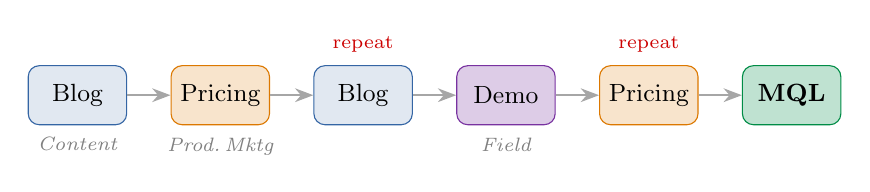
\begin{tikzpicture}[node distance=0.55cm]
  \node[blognode] (a) {Blog};
  \node[pricenode, right=of a] (b) {Pricing};
  \node[blognode, right=of b] (c) {Blog};
  \node[demonode, right=of c] (d) {Demo};
  \node[pricenode, right=of d] (e) {Pricing};
  \node[mqlnode, right=of e] (f) {MQL};
  \foreach \i/\j in {a/b,b/c,c/d,d/e,e/f} \draw[jarrow] (\i) -- (\j);
  \node[font=\scriptsize\itshape, gray, below=1pt of a] {Content};
  \node[font=\scriptsize\itshape, gray, below=1pt of b] {Prod.\,Mktg};
  \node[font=\scriptsize\itshape, gray, below=1pt of d] {Field};
  \node[font=\scriptsize, sampred, above=1pt of c] {repeat};
  \node[font=\scriptsize, sampred, above=1pt of e] {repeat};
\end{tikzpicture}

\vspace{1.0em}
{\small 5 touchpoints, but only \textbf{3 distinct channels} --- Blog, Pricing, Demo.}
\end{frame}

\begin{frame}{Three teams, three assets}
\vspace{0.3em}
\centering
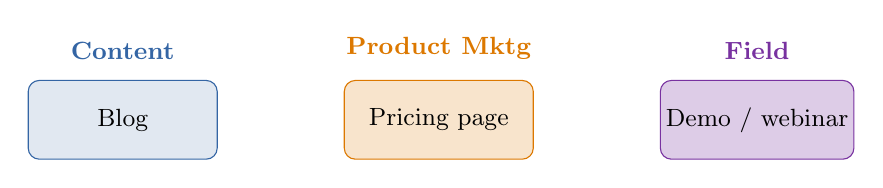
\begin{tikzpicture}[node distance=1.6cm]
  \node[blognode, minimum width=2.4cm, minimum height=1.0cm] (b) {Blog};
  \node[pricenode, minimum width=2.4cm, minimum height=1.0cm, right=of b] (p) {Pricing page};
  \node[demonode, minimum width=2.4cm, minimum height=1.0cm, right=of p] (d) {Demo / webinar};
  \node[above=4pt of b, font=\small\bfseries, popblue] {Content};
  \node[above=4pt of p, font=\small\bfseries, orange1] {Product Mktg};
  \node[above=4pt of d, font=\small\bfseries, violet1] {Field};
\end{tikzpicture}

\vspace{1.0em}
Each team asks the same question:\\[3pt]
{\large\itshape ``Did \emph{my} asset drive the MQL?''}

\vspace{1.0em}
\textcolor{warnred}{\textbf{Budget and headcount ride on the answer.}}
\end{frame}

\begin{frame}{5 touches, 1 conversion --- who gets the credit?}
\centering
\vspace{0.6em}
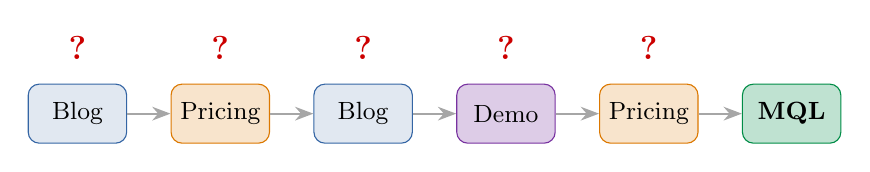
\begin{tikzpicture}[node distance=0.55cm]
  \node[blognode] (a) {Blog};
  \node[pricenode, right=of a] (b) {Pricing};
  \node[blognode, right=of b] (c) {Blog};
  \node[demonode, right=of c] (d) {Demo};
  \node[pricenode, right=of d] (e) {Pricing};
  \node[mqlnode, right=of e] (f) {MQL};
  \foreach \i/\j in {a/b,b/c,c/d,d/e,e/f} \draw[jarrow] (\i)--(\j);
  \foreach \n in {a,b,c,d,e} \node[above=5pt of \n, sampred, font=\large\bfseries] {?};
\end{tikzpicture}

\vspace{1.0em}
We must split \textbf{one} conversion's credit across the channels that led to it.\\[4pt]
{\small How much of the MQL does each of Blog, Pricing, Demo deserve?}
\end{frame}

\begin{frame}{We see \emph{that} they converted, not \emph{why}}
\vspace{0.4em}
\begin{itemize}
  \itemsep0.7em
  \item The data shows the touches and the outcome --- not the cause.
  \item A channel being \emph{present} in winning journeys $\neq$ that channel \emph{caused} the win.
  \item Popular channels look good simply by appearing everywhere.
\end{itemize}
\vspace{0.8em}
\centering\textcolor{popblue}{So: how do we turn ``was present'' into ``deserves credit''?}
\end{frame}

\begin{frame}{Attribution = a share of credit per channel}
\vspace{0.3em}
\begin{block}{Goal}
Assign each channel a \textbf{credit} number, so the shares are comparable --- which assets actually move MQLs.
\end{block}
\vspace{0.4em}
\begin{itemize}
  \itemsep0.4em
  \item Bigger credit $\Rightarrow$ that channel was more responsible for conversions.
  \item Lets each team see the return on its work.
\end{itemize}
\end{frame}

\begin{frame}{From messy journey to distinct channels}
\centering
\vspace{0.2em}
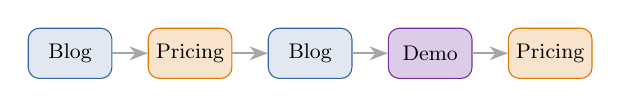
\begin{tikzpicture}[node distance=0.45cm]
  \node[blognode, scale=0.85] (a) {Blog};
  \node[pricenode, scale=0.85, right=of a] (b) {Pricing};
  \node[blognode, scale=0.85, right=of b] (c) {Blog};
  \node[demonode, scale=0.85, right=of c] (d) {Demo};
  \node[pricenode, scale=0.85, right=of d] (e) {Pricing};
  \foreach \i/\j in {a/b,b/c,c/d,d/e} \draw[jarrow] (\i)--(\j);
\end{tikzpicture}

\vspace{0.2em}
{\small For now, \emph{for simplicity}, we collapse to the \emph{set} of distinct channels} $\big\downarrow$

\vspace{0.3em}
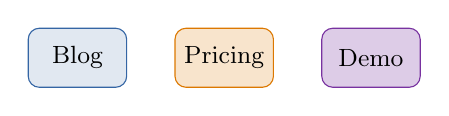
\begin{tikzpicture}[node distance=0.6cm]
  \node[blognode] (a) {Blog};
  \node[pricenode, right=of a] (b) {Pricing};
  \node[demonode, right=of b] (d) {Demo};
\end{tikzpicture}

\vspace{0.6em}
\callout{\textbf{We just threw away the repeats} --- Blog and Pricing were each hit twice. \textbf{Hold that thought.}}
\end{frame}

% ============================================================
% SECTION 2 - HEURISTIC RULES
% ============================================================

\begin{frame}{First touch vs last touch}
\centering
This journey --- which single channel deserves the credit?
\vspace{0.2em}

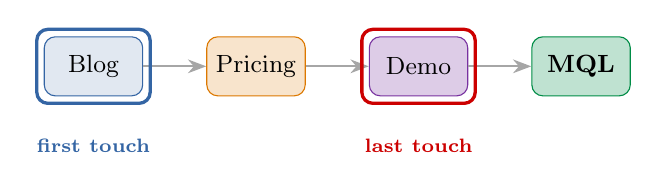
\begin{tikzpicture}[node distance=0.8cm]
  \node[blognode] (a) {Blog};
  \node[pricenode, right=of a] (b) {Pricing};
  \node[demonode, right=of b] (d) {Demo};
  \node[mqlnode, right=of d] (f) {MQL};
  \foreach \i/\j in {a/b,b/d,d/f} \draw[jarrow] (\i)--(\j);
  \node<2->[draw=popblue, very thick, rounded corners, fit=(a), inner sep=2.5pt]{};
  \node<2->[below=12pt of a, popblue, font=\scriptsize\bfseries] {first touch};
  \node<2->[draw=sampred, very thick, rounded corners, fit=(d), inner sep=2.5pt]{};
  \node<2->[below=12pt of d, sampred, font=\scriptsize\bfseries] {last touch};
\end{tikzpicture}

\onslide<2->{\par\vspace{0.4em}\textbf{First-touch} credits \textcolor{popblue}{Blog}. \quad \textbf{Last-touch} credits \textcolor{sampred}{Demo}. \quad \textcolor{warnred}{\textbf{Opposite!}}}

\onslide<3->{
\par\vspace{0.3em}{\small Apply each rule across \emph{all} journeys $\Rightarrow$ channel-level credit:}\\[2pt]
\begin{columns}[T]
\column{0.46\textwidth}\centering {\scriptsize first-touch}\\[2pt] \creditbars{57}{29}{14}
\column{0.46\textwidth}\centering {\scriptsize last-touch}\\[2pt] \creditbars{14}{29}{57}
\end{columns}}
\end{frame}

\begin{frame}{Each single-touch rule has a built-in bias}
\vspace{0.5em}
\begin{columns}[T]
\column{0.5\textwidth}
\textbf{\textcolor{popblue}{First-touch}}
\begin{itemize}\small
  \itemsep0.4em
  \item Over-credits \emph{top-of-funnel} --- awareness, discovery.
  \item Ignores everything that nurtured and closed.
\end{itemize}
\column{0.5\textwidth}
\textbf{\textcolor{sampred}{Last-touch}}
\begin{itemize}\small
  \itemsep0.4em
  \item Over-credits \emph{the closer} --- the final click.
  \item Ignores what built the interest in the first place.
\end{itemize}
\end{columns}
\vspace{1.0em}
\centering\textcolor{warnred}{Either way: you reward one touch and erase the rest.}
\end{frame}

\begin{frame}{Spreading the credit: multi-touch rules}
\centering
Give \emph{every} touch some credit --- but how much? \\[2pt]
{\small (positions on the journey Blog $\to$ Pricing $\to$ Demo)}
\vspace{0.7em}

\begin{columns}[T]
\column{0.33\textwidth}\centering \textbf{Linear}\\[1pt]{\scriptsize equal split}\\[5pt]\creditbars{33}{33}{33}
\column{0.33\textwidth}\centering \textbf{Time-decay}\\[1pt]{\scriptsize recent weighted}\\[5pt]\creditbars{20}{30}{50}
\column{0.33\textwidth}\centering \textbf{U-shaped}\\[1pt]{\scriptsize ends weighted}\\[5pt]\creditbars{40}{20}{40}
\end{columns}
\vspace{0.7em}
{\small Each is a fixed \emph{position-based} recipe --- it never looks at the outcomes.}
\end{frame}

\begin{frame}{Why 40/40/20, and not 30/30/40?}
\vspace{0.5em}
\callout{These splits are \textbf{arbitrary} --- picked by hand, justified by \emph{nothing in the data}.}
\vspace{0.2em}
\begin{itemize}\small
  \itemsep0.4em
  \item Every rule so far decides credit by \emph{position}, before looking at outcomes.
  \item Change the recipe, change the ``winner'' --- with no principled way to choose.
\end{itemize}
\vspace{0.4em}
\callout[popblue]{\textbf{Data-driven idea:} let the \emph{data} decide --- which channels actually move conversions?}
\end{frame}

% ============================================================
% SECTION 3 - MARKOV CHAINS
% ============================================================

\begin{frame}{A Markov chain in one picture}
\centering
\vspace{0.2em}
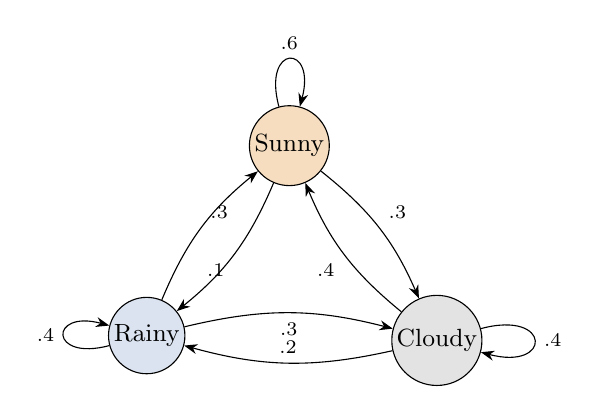
\begin{tikzpicture}[node distance=2.8cm]
  \node[statenode, fill=orange1!25] (s) {Sunny};
  \node[statenode, fill=popblue!18, below left=1.7cm and 1.1cm of s] (r) {Rainy};
  \node[statenode, fill=gray!22, below right=1.7cm and 1.1cm of s] (c) {Cloudy};
  \draw[-{Stealth}] (s) to[bend left=14] node[above right,font=\scriptsize]{.3} (c);
  \draw[-{Stealth}] (c) to[bend left=14] node[below left,font=\scriptsize]{.4} (s);
  \draw[-{Stealth}] (s) to[bend left=14] node[below left,font=\scriptsize]{.1} (r);
  \draw[-{Stealth}] (r) to[bend left=14] node[above right,font=\scriptsize]{.3} (s);
  \draw[-{Stealth}] (r) to[bend left=14] node[below,font=\scriptsize]{.3} (c);
  \draw[-{Stealth}] (c) to[bend left=14] node[above,font=\scriptsize]{.2} (r);
  \draw[-{Stealth}] (s) to[loop above] node[font=\scriptsize]{.6} (s);
  \draw[-{Stealth}] (r) to[loop left] node[font=\scriptsize]{.4} (r);
  \draw[-{Stealth}] (c) to[loop right] node[font=\scriptsize]{.4} (c);
\end{tikzpicture}

\vspace{0.5em}
{\small \textbf{States} + \textbf{transition probabilities}. Each arrow: ``given today, the chance of tomorrow.''}
\end{frame}

\begin{frame}{From one state, the chances sum to 1}
\centering
{\small Given \textbf{today is Sunny}, tomorrow is exactly one of:}
\vspace{0.3em}

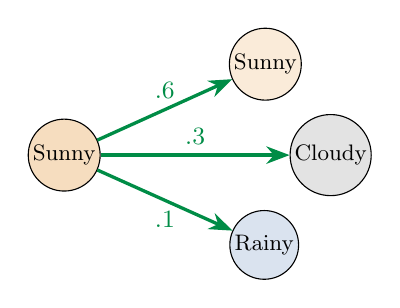
\begin{tikzpicture}[node distance=1.8cm]
  \node[statenode, scale=0.9, fill=orange1!25] (s) {Sunny};
  \node[statenode, scale=0.9, fill=orange1!15, above right=0.5cm and 1.9cm of s] (s2) {Sunny};
  \node[statenode, scale=0.9, fill=gray!22, right=2.4cm of s] (c) {Cloudy};
  \node[statenode, scale=0.9, fill=popblue!18, below right=0.5cm and 1.9cm of s] (r) {Rainy};
  \draw[-{Stealth}, very thick, paramgreen] (s) -- (s2) node[midway,above,font=\small]{.6};
  \draw[-{Stealth}, very thick, paramgreen] (s) -- (c) node[midway,above,font=\small]{.3};
  \draw[-{Stealth}, very thick, paramgreen] (s) -- (r) node[midway,below,font=\small]{.1};
\end{tikzpicture}

\vspace{0.3em}
\[ \underbrace{0.6}_{\text{Sunny}} + \underbrace{0.3}_{\text{Cloudy}} + \underbrace{0.1}_{\text{Rainy}} = 1 \]
\callout[popblue]{From any state, the outgoing arrows cover every option --- they \textbf{always sum to 1}.}
\end{frame}

\begin{frame}{Memoryless: only \emph{now} matters}
\vspace{0.4em}
\begin{block}{The Markov property}
The next state depends \textbf{only on the current state} --- not on the full history of how you got there.
\end{block}
\vspace{0.5em}
\centering{\small Weather: tomorrow depends on today, not on what happened last week.}
\vspace{0.9em}
\callout[gray]{Real journeys \emph{do} have memory --- first-order Markov is a deliberate simplification. (Higher-order chains exist; we keep it first-order here.)}
\end{frame}

\begin{frame}{A journey is a walk through channel-states}
\centering
\vspace{0.2em}
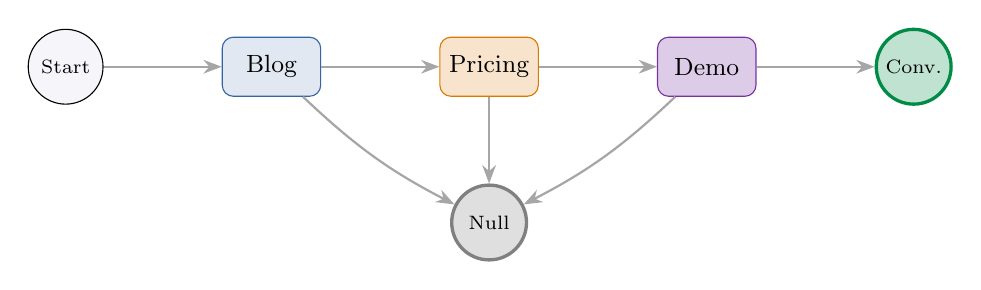
\begin{tikzpicture}[node distance=1.3cm and 1.5cm]
  \node[statenode, fill=lightbg] (st) {\scriptsize Start};
  \node[blognode] (b) [right=of st] {Blog};
  \node[pricenode] (p) [right=of b] {Pricing};
  \node[demonode] (d) [right=of p] {Demo};
  \node[absorb, fill=paramgreen!25, draw=paramgreen] (cv) [right=of d] {\scriptsize Conv.};
  \node[absorb, fill=gray!25, draw=gray] (nl) [below=1.1cm of p] {\scriptsize Null};
  \draw[jarrow] (st)--(b); \draw[jarrow] (b)--(p); \draw[jarrow] (p)--(d); \draw[jarrow] (d)--(cv);
  \draw[jarrow] (b) to[bend right=8] (nl); \draw[jarrow] (p)--(nl); \draw[jarrow] (d) to[bend left=8] (nl);
\end{tikzpicture}

\vspace{0.7em}
\begin{itemize}\small
  \itemsep0.3em
  \item States = the channels, plus \textbf{Start}, \textbf{Convert}, and \textbf{Null} (no conversion).
  \item \textcolor{paramgreen}{\textbf{Convert}} and \textcolor{gray}{\textbf{Null}} are \emph{absorbing}: once you arrive, you stay.
\end{itemize}
\end{frame}

\begin{frame}{Estimate transition probabilities by counting}
\vspace{0.6em}
\begin{columns}[c]
\column{0.5\textwidth}
\centering
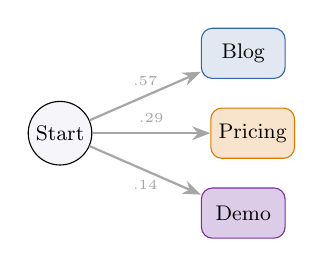
\begin{tikzpicture}[node distance=0.9cm and 1.5cm, every node/.style={font=\scriptsize}]
  \node[statenode, fill=lightbg, scale=0.85] (st) {Start};
  \node[blognode, scale=0.85] (b) [above right=0.4cm and 1.5cm of st] {Blog};
  \node[pricenode, scale=0.85] (p) [right=1.5cm of st] {Pricing};
  \node[demonode, scale=0.85] (d) [below right=0.4cm and 1.5cm of st] {Demo};
  \draw[jarrow] (st)--(b) node[midway,above,font=\tiny]{.57};
  \draw[jarrow] (st)--(p) node[midway,above,font=\tiny]{.29};
  \draw[jarrow] (st)--(d) node[midway,below,font=\tiny]{.14};
\end{tikzpicture}
\column{0.5\textwidth}
\small Count transitions; divide by row totals. The \textbf{Start} row from our data:
\[ \text{Start}\!\to\!(\text{B},\text{P},\text{D}) = (.57,\ .29,\ .14) \]
{\scriptsize Every state's outgoing probabilities sum to 1.}
\end{columns}
\end{frame}

\begin{frame}{How likely is conversion? Add up the paths}
\vspace{0.2em}
\begin{columns}[c]
\column{0.5\textwidth}
\centering
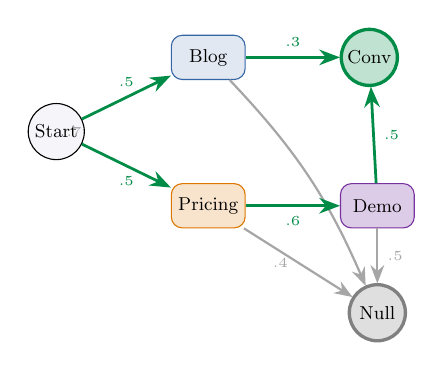
\begin{tikzpicture}[node distance=0.8cm and 1.2cm, every node/.style={font=\scriptsize}]
  \node[statenode, fill=lightbg, scale=0.75] (st) {Start};
  \node[blognode, scale=0.75] (b) [above right=0.4cm and 1.2cm of st] {Blog};
  \node[pricenode, scale=0.75] (p) [below right=0.4cm and 1.2cm of st] {Pricing};
  \node[demonode, scale=0.75] (d) [right=1.2cm of p] {Demo};
  \node[absorb, fill=paramgreen!25, draw=paramgreen, scale=0.75] (cv) [right=1.2cm of b] {Conv};
  \node[absorb, fill=gray!25, draw=gray, scale=0.75] (nl) [below=0.7cm of d] {Null};
  \draw[-{Stealth}, paramgreen, line width=1pt] (st)--(b) node[midway,above,font=\tiny]{.5};
  \draw[-{Stealth}, paramgreen, line width=1pt] (st)--(p) node[midway,below,font=\tiny]{.5};
  \draw[-{Stealth}, paramgreen, line width=1pt] (b)--(cv) node[midway,above,font=\tiny]{.3};
  \draw[jarrow] (b) to[bend left=10] (nl) node[pos=0.3,right,font=\tiny]{.7};
  \draw[-{Stealth}, paramgreen, line width=1pt] (p)--(d) node[midway,below,font=\tiny]{.6};
  \draw[jarrow] (p)--(nl) node[pos=0.5,left,font=\tiny]{.4};
  \draw[-{Stealth}, paramgreen, line width=1pt] (d)--(cv) node[pos=0.5,right,font=\tiny]{.5};
  \draw[jarrow] (d)--(nl) node[midway,right,font=\tiny]{.5};
\end{tikzpicture}\\[2pt]
{\scriptsize illustrative acyclic graph --- \textcolor{paramgreen}{green = converting paths}}
\column{0.5\textwidth}
\small
\[ P(\text{conv}) = \!\!\sum_{\text{Start}\to\cdots\to\text{Conv}}\ \prod_{\text{edges}} p \]
Two converting paths:
\begin{itemize}\scriptsize
  \item St$\to$Blog$\to$Conv: $.5\times.3=.15$
  \item St$\to$Pric$\to$Demo$\to$Conv: $.5\times.6\times.5=.15$
\end{itemize}
\[ P(\text{conv}) = .15+.15 = \mathbf{0.30} \]
\end{columns}
\vspace{0.2em}
\callout[gray]{With repeat visits (cycles) the paths are infinite --- use the \emph{fundamental matrix}. The script does this for the real numbers.}
\end{frame}

\begin{frame}{Remove a channel, watch conversion drop}
\vspace{0.4em}
\begin{block}{Removal effect = a channel's importance}
\[ \text{credit}_i \ \propto\ \frac{P(\text{convert}) - P(\text{convert}\mid i\text{ removed})}{P(\text{convert})} \]
\end{block}
\vspace{0.2em}
\begin{itemize}\small
  \itemsep0.3em
  \item \textbf{Remove a channel} = redirect all its incoming transitions to \textbf{Null}.
  \item The bigger the drop in conversion, the more that channel mattered.
  \item Compute for every channel, then normalize to shares.
\end{itemize}
\end{frame}

\begin{frame}{Removing Pricing}
\centering
\vspace{0.4em}
\begin{columns}[c]
\column{0.5\textwidth}\centering {\scriptsize full chain}\\[2pt] $P(\text{conv}) = \mathbf{0.386}$
\column{0.5\textwidth}\centering {\scriptsize Pricing\,$\to$\,Null}\\[2pt] $P(\text{conv}) = \mathbf{0.157}$
\end{columns}
\vspace{0.5em}
\[ \text{removal effect}_{\text{Pricing}} = \frac{0.386-0.157}{0.386} \approx 0.59 \quad(\text{a 59\% drop}) \]
\vspace{0.1em}
\centering{\small Repeat for all three, normalize $\Rightarrow$ Markov credit shares:}\\[4pt]
\creditbars{28}{32}{40}
\end{frame}

\begin{frame}{Markov's question}
\vspace{1.2em}
\callout[popblue]{\large Markov asks:\\[6pt] \emph{``What \textbf{breaks} if this channel disappears?''}}
\vspace{0.8em}
\centering{\small A natural ``what if we turned it off?'' view of importance.}
\vspace{0.7em}

\textcolor{gray}{Next: a completely different question --- \emph{fairness}.}
\end{frame}

% ============================================================
% SECTION 4 - SHAPLEY VALUE
% ============================================================

\begin{frame}{Three people close one deal --- split the bonus fairly}
\centering
\vspace{0.5em}
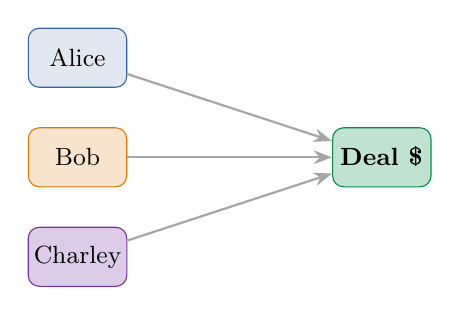
\begin{tikzpicture}[node distance=0.5cm]
  \node[chnode, fill=popblue!15, draw=popblue] (sdr) {Alice};
  \node[chnode, fill=orange1!20, draw=orange1, below=of sdr] (ae) {Bob};
  \node[chnode, fill=violet1!25, draw=violet1, below=of ae] (se) {Charley};
  \node[mqlnode, right=2.6cm of ae] (deal) {Deal \$};
  \draw[jarrow] (sdr)--(deal); \draw[jarrow] (ae)--(deal); \draw[jarrow] (se)--(deal);
\end{tikzpicture}

\vspace{0.6em}
They produced \textbf{one} outcome \emph{together}.\\[3pt]
{\large What is each person's \textcolor{paramgreen}{fair share} of the bonus?}

\vspace{0.5em}
\callout[popblue]{Channels are the same: several touches jointly produce \textbf{one} conversion.}
\end{frame}

\begin{frame}{Average marginal contribution over all join orders}
\vspace{0.3em}
\begin{itemize}\small
  \itemsep0.4em
  \item Imagine the players joining a team \emph{one at a time}.
  \item A player's \textbf{marginal contribution} = how much value they \emph{add} when they join.
  \item \textbf{Shapley value} = that contribution, \emph{averaged over every possible order}.
\end{itemize}
\vspace{0.5em}
\centering
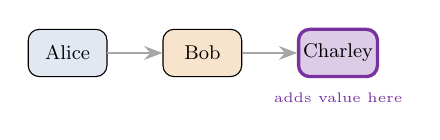
\begin{tikzpicture}[node distance=0.7cm, every node/.style={font=\scriptsize}]
  \node[chnode, scale=0.8, fill=popblue!15] (a) {Alice};
  \node[chnode, scale=0.8, fill=orange1!20, right=of a] (b) {Bob};
  \node[chnode, scale=0.8, fill=violet1!25, draw=violet1, very thick, right=of b] (c) {Charley};
  \draw[jarrow] (a)--(b); \draw[jarrow] (b)--(c);
  \node[below=2pt of c, violet1, font=\tiny] {adds value here};
\end{tikzpicture}\\
{\scriptsize one ordering: Alice, then Bob, then Charley --- measure what Charley adds}
\end{frame}

\begin{frame}{All 6 orders --- Blog's marginal contribution}
\centering
{\small $v(S)$ = conversion rate of journeys with exactly set $S$.}\\[5pt]
\begin{tabular}{llc}
\toprule
order & set before Blog & Blog adds \\
\midrule
B, P, D & $\varnothing$ & $v(B)-0 = .10$ \\
B, D, P & $\varnothing$ & $.10$ \\
P, B, D & $\{P\}$ & $v(BP)-v(P)=.20$ \\
D, B, P & $\{D\}$ & $v(BD)-v(D)=.15$ \\
P, D, B & $\{P,D\}$ & $v(BPD)-v(PD)=.15$ \\
D, P, B & $\{P,D\}$ & $.15$ \\
\bottomrule
\end{tabular}\\[5pt]
{\small Six ``what does Blog add'' numbers --- one per order.}
\end{frame}

\begin{frame}{Average them = Shapley value}
\centering
\vspace{0.4em}
\[ \phi_{\text{Blog}} = \frac{.10+.10+.20+.15+.15+.15}{6} = \frac{0.85}{6} \approx 0.142 \]
\vspace{0.2em}
Same averaging for each channel:
\[ \phi_{\text{Blog}}\approx.142,\qquad \phi_{\text{Pricing}}\approx.242,\qquad \phi_{\text{Demo}}\approx.317 \]
\vspace{0.1em}
\[ \underbrace{.142+.242+.317}_{\text{the three Shapley values}} \;=\; \underbrace{0.70}_{v(\{B,P,D\})} \]
{\small $v(\{B,P,D\})$ = conversion value of all three channels together.}
\callout[paramgreen]{Efficiency: the credits add up to the whole --- \textbf{no credit lost or invented.}}
\end{frame}

\begin{frame}{The same thing, written compactly}
\vspace{0.6em}
\[ \phi_i = \sum_{S \subseteq N\setminus\{i\}} \frac{|S|!\,(|N|-|S|-1)!}{|N|!}\,\bigl(v(S\cup\{i\}) - v(S)\bigr) \]
\vspace{0.4em}
\begin{itemize}\small
  \itemsep0.3em
  \item The sum runs over every subset $S$ that could be ``already there'' before $i$ joins.
  \item The fraction is just the weight that makes \emph{every join order equally likely}.
  \item Exactly the average we did by hand --- now in one line.
\end{itemize}
\end{frame}

\begin{frame}{Why Shapley? It's the \emph{only} fair split}
\vspace{0.3em}
A wishlist any fair credit rule should satisfy:
\begin{itemize}\small
  \itemsep0.35em
  \item \textbf{Efficiency} --- the credits add up to the total value.
  \item \textbf{Symmetry} --- equal contributors get equal credit.
  \item \textbf{Null player} --- a channel that adds nothing gets zero.
  \item \textbf{Additivity} --- credit adds up across combined games.
\end{itemize}
\vspace{0.5em}
\callout[popblue]{Shapley is the \textbf{unique} rule satisfying all four.}
\end{frame}

\begin{frame}{Channels as players}
\centering
\vspace{0.3em}
$v(S) = $ conversion rate of journeys whose distinct channel set is \textbf{exactly} $S$.
\vspace{0.7em}

{\small Predict: which channel earns the most credit?}
\pause
\vspace{0.4em}

\creditbars{20}{35}{45}\\[2pt]{\scriptsize Shapley credit}
\vspace{0.4em}
\callout{First-touch crowned \textbf{Blog} (57\%). Shapley says Blog earns just \textbf{20\%} --- \textbf{Demo} is the real driver.}
\end{frame}

\begin{frame}{The catch: $2^n$ coalitions}
\vspace{0.4em}
\begin{itemize}\small
  \itemsep0.4em
  \item With $n$ channels there are $2^n$ subsets to value.
  \item 3 channels $\to$ 8 subsets (easy). 20 channels $\to$ over a million.
  \item Exact Shapley gets expensive fast $\Rightarrow$ in practice, \emph{sample} orderings / approximate.
\end{itemize}
\vspace{0.7em}
\callout[popblue]{This cost --- and the need for richer features --- points to \textbf{Shapley on top of ML}.}
\end{frame}

% ============================================================
% SECTION 5 - SHAPLEY ON TOP OF ML (SHAP)
% ============================================================

\begin{frame}{Raw Shapley sees only presence}
\vspace{0.5em}
\begin{itemize}\small
  \itemsep0.5em
  \item It uses only \emph{which} channels were present --- a 0/1 flag per channel.
  \item Rare channel combinations have little or no data $\Rightarrow$ $v(S)$ is noisy or undefined.
  \item We want \textbf{richer features} and a way to \textbf{fill the gaps}.
\end{itemize}
\vspace{0.8em}
\centering\textcolor{popblue}{Idea: let a \emph{model} estimate $v(S)$ instead of raw counts.}
\end{frame}

\begin{frame}{Same math, a new value function}
\vspace{0.3em}
\begin{columns}[T]
\column{0.5\textwidth}
\centering\textbf{\textcolor{popblue}{\S4: empirical}}\\[4pt]
\fcolorbox{popblue}{popblue!8}{\parbox{0.88\linewidth}{\centering\small $v(S)=$ conversion rate \emph{counted from data} for set $S$}}
\column{0.5\textwidth}
\centering\textbf{\textcolor{paramgreen}{\S5: model}}\\[4pt]
\fcolorbox{paramgreen}{paramgreen!8}{\parbox{0.88\linewidth}{\centering\small $v(S)=$ the model's \emph{predicted} conversion prob.\ using only the features in $S$}}
\end{columns}
\vspace{0.7em}
\callout[popblue]{Same Shapley formula --- the value function goes from \emph{counted-from-data} to \emph{model-predicted}.}
\centering{\small Why it helps: the model \textbf{interpolates} channel combinations the raw counts never saw.}\\[4pt]
{\large This is \textbf{SHAP} --- SHapley Additive exPlanations.}
\end{frame}

\begin{frame}{From journeys to SHAP credit}
\centering
\vspace{0.8em}
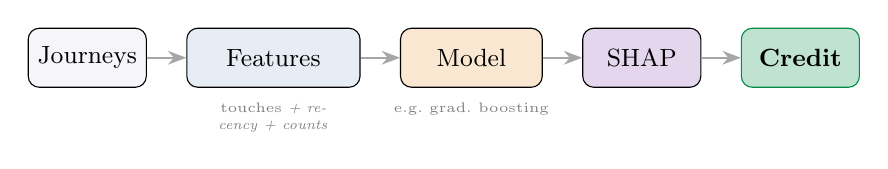
\begin{tikzpicture}[node distance=0.5cm, every node/.style={font=\scriptsize}]
  \node[chnode, fill=lightbg, minimum width=1.5cm] (j) {Journeys};
  \node[chnode, fill=popblue!12, minimum width=2.2cm, right=of j] (f) {Features};
  \node[chnode, fill=orange1!18, minimum width=1.8cm, right=of f] (m) {Model};
  \node[chnode, fill=violet1!20, minimum width=1.5cm, right=of m] (s) {SHAP};
  \node[mqlnode, minimum width=1.5cm, right=of s] (c) {Credit};
  \foreach \i/\j in {j/f,f/m,m/s,s/c} \draw[jarrow] (\i)--(\j);
  \node[below=2pt of f, gray, font=\tiny, text width=2.3cm, align=center] {touches \emph{+ recency + counts}};
  \node[below=2pt of m, gray, font=\tiny] {e.g.\ grad.\ boosting};
\end{tikzpicture}

\vspace{1.1em}
{\small Features can now go \emph{beyond} 0/1 --- recency, frequency, dwell, and more.}
\end{frame}

\begin{frame}{From one prediction to channel-level credit}
\vspace{0.4em}
\begin{itemize}\small
  \itemsep0.4em
  \item SHAP explains \emph{one user's} predicted probability --- splitting it across that user's features.
  \item Average $|\text{SHAP}|$ across all users $\Rightarrow$ aggregate channel credit.
\end{itemize}
\vspace{0.4em}
\centering
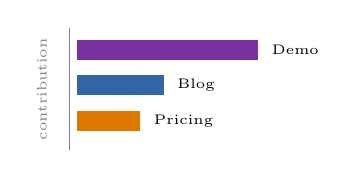
\begin{tikzpicture}[every node/.style={font=\scriptsize}, x=1cm, y=0.5cm]
  \draw[gray] (0.3,0) -- (0.3,3.1);
  \node[rotate=90, gray, font=\tiny] at (-0.05,1.55) {contribution};
  \fill[violet1] (0.4,2.3) rectangle (2.7,2.8); \node[right,font=\tiny] at (2.75,2.55){Demo};
  \fill[popblue] (0.4,1.4) rectangle (1.5,1.9); \node[right,font=\tiny] at (1.55,1.65){Blog};
  \fill[orange1] (0.4,0.5) rectangle (1.2,1.0); \node[right,font=\tiny] at (1.25,0.75){Pricing};
\end{tikzpicture}\\
{\scriptsize one journey's SHAP contributions to its predicted conversion probability}
\end{frame}

% ============================================================
% SECTION 6 - LIMITATIONS
% ============================================================

\begin{frame}{Everything so far treats a touch as 0/1}
\vspace{0.3em}
\callout{Remember the repeated Blog and Pricing visits we dropped on slide 1? That's \textbf{frequency} --- gone.}
\vspace{0.1em}
Also invisible to these models:
\begin{itemize}\small
  \itemsep0.25em
  \item \textbf{Recency} --- how recently each touch happened.
  \item \textbf{Repetition} --- one visit vs ten.
\end{itemize}
\vspace{0.2em}
\centering
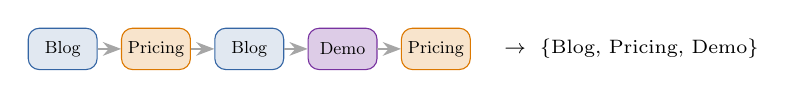
\begin{tikzpicture}[node distance=0.3cm, every node/.style={font=\tiny}]
  \node[blognode, scale=0.7] (a) {Blog};
  \node[pricenode, scale=0.7, right=of a] (b) {Pricing};
  \node[blognode, scale=0.7, right=of b] (c) {Blog};
  \node[demonode, scale=0.7, right=of c] (d) {Demo};
  \node[pricenode, scale=0.7, right=of d] (e) {Pricing};
  \foreach \i/\j in {a/b,b/c,c/d,d/e} \draw[jarrow] (\i)--(\j);
  \node[right=0.3cm of e, font=\scriptsize] {$\to\ \{$Blog, Pricing, Demo$\}$};
\end{tikzpicture}
\end{frame}

\end{document}
